Using pytorch \cite{pytorch} several models are constructed, trained and evaluated.

\subsection{Data}\label{subsec:data}
Archive of Motion Capture as Surface Shapes (AMASS) \cite{AMASS:2019} is a collection of motion capture datasets. An example of a motion capture visualization can be seen in \autoref{fig:walking}. AMASS collects several datasets into one single place and unifies the data format to a single data format. All models will be trained on data AMASS. Specifically all data from the CMU \cite{cmuWEB} dataset (part of AMASS) that has been tagged with the \texttt{walk} tag. Motion is usually stored as rotations around joints, as human limbs generally speaking only rotate and do not stretch. This means that most motions consist only of rotations and a root position. Only the rotational data is used in order to simplify the different types of data the models are trained on. Some visualizations in this paper include root position, when that is the case the root position is always the reference root position.

In order to visualize motion a skeleton is needed. A skeleton is mostly just where the joints are positioned relative to each other and a mesh. For this the skeleton from \cite{MANO} is used. This paper only visualizes the joints, the mesh is never used in visualization.

In order to load in the motion data the library fairmotion \cite{gopinath2020fairmotion} is used. It provides an easy way to load and manipulate motion data and is also the tool used for visualization.


\begin{figure}[h]
\centering
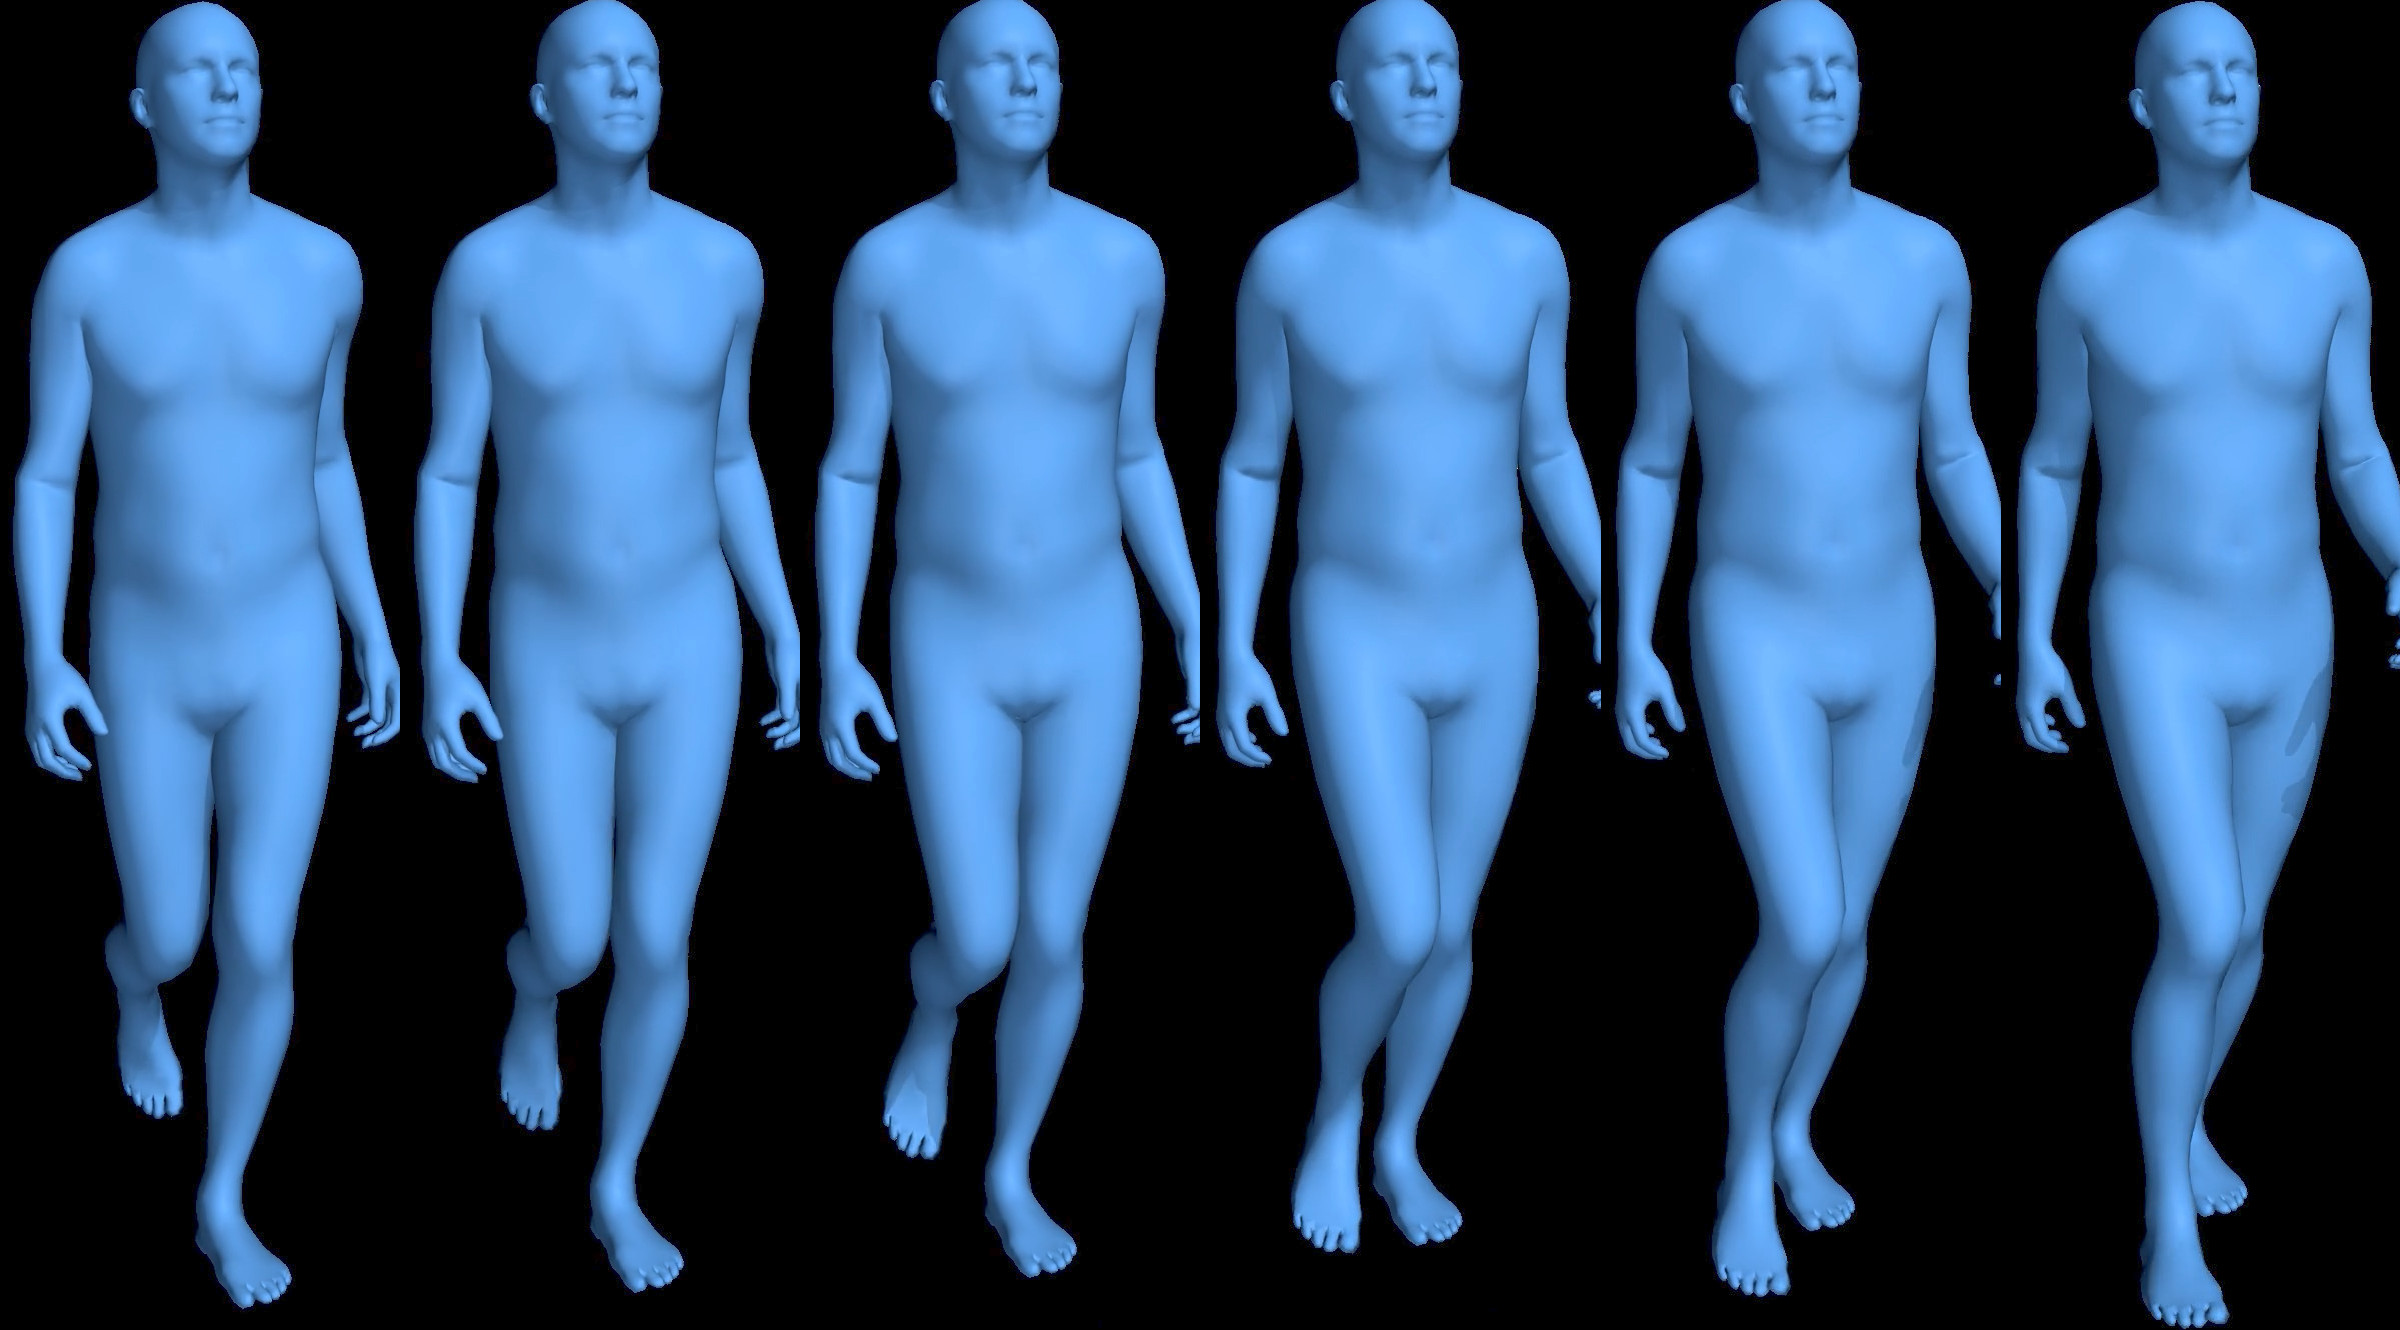
\includegraphics[width=0.3\textwidth]{img/02_01}
\caption{Small snippet of a walking motion from the AMASS dataset.}
\label{fig:walking}
\end{figure}



\subsection{Models}\label{subsec:models}
An autoencoder consists of an encoder and a decoder. The encoder works by taking an input and then encoding it into a smaller space called the latent space. The encoder then decodes the latent value back into something similar to the original input value. Such an operation by itself is pointless, but by doing this we are forcing the model to learn which features of the input are necessary for faithful reconstruction and which features can be discarded. This essentially gives us a compressed version of the input, where each change in the latent space is likely to be clearly visible in the output, similar to principal components analysis~\cite{TODO}.An autoencoder consists of an encoder and a decoder. The encoder works by taking an input and then encoding it into a smaller space called the latent space. The encoder then decodes the latent value back into something similar to the original input value. Such an operation by itself is pointless, but by doing this we are forcing the model to learn which features of the input are necessary for faithful reconstruction and which features can be discarded. This essentially gives us a compressed version of the input, where each change in the latent space is likely to be clearly visible in the output, similar to principal components analysis~\cite{TODO}.


\begin{figure}[h]
\centering
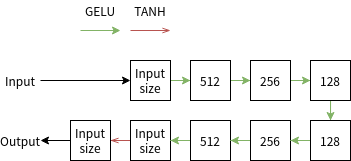
\includegraphics[width=0.5\textwidth]{img/autoencoder}
\caption{Diagram of the model used to implement a simple autoencoder. Each arrow represents a linear layer with either the GELU or tanh activation function applied to its output.}
\label{fig:autoencoder}
\end{figure}

A simple autoencoder using decreasingly smaller/increasingly larger hidden layers for encoding/decoding can be seen in \autoref{fig:autoencoder}. This will be used as a baseline of comparison against the VAE.

Since the above model is bad (non-continuous) we actually want to use a VAE which, TODO: describe VAE and my implementation.

\subsection{Training}\label{subsec:training}
notes on how the training was performed